
With the advent of technologies that make access to information
scalable and affordable, the mental and temporal gap between
collection of data and their analysis grows rapidly. At least two of
the biggest players in the the tech industry, Facebook and Google,
base their competitive advantage on vast amounts of information that
they have collected and their capacity for such collection. In cases
like these the layout of the stored data is independent of the growing
number of applications taking advantage of it. We believe there are
opportunities in automatically and dynamically optimizing data
representation to fit the workload.

Consider the following query over the TPC-H dataset that computes the average discount per country:

\begin{code}
  \begin{sqlcode}
    select      n_name, avg(l_discount)
    from        lineitem, customer, nation, order
    where       l_orderkey = o_orderkey
    and         c_custkey = o_custkey
    and         c_nationkey = n_nationkey
    and         l_shipdate > 10-11-2015
    group by    n_name
  \end{sqlcode}
\end{code}

An optimizer considering this query in isolation might come up with
the following plan following plan:

\begin{figure}[H]
  \centering
  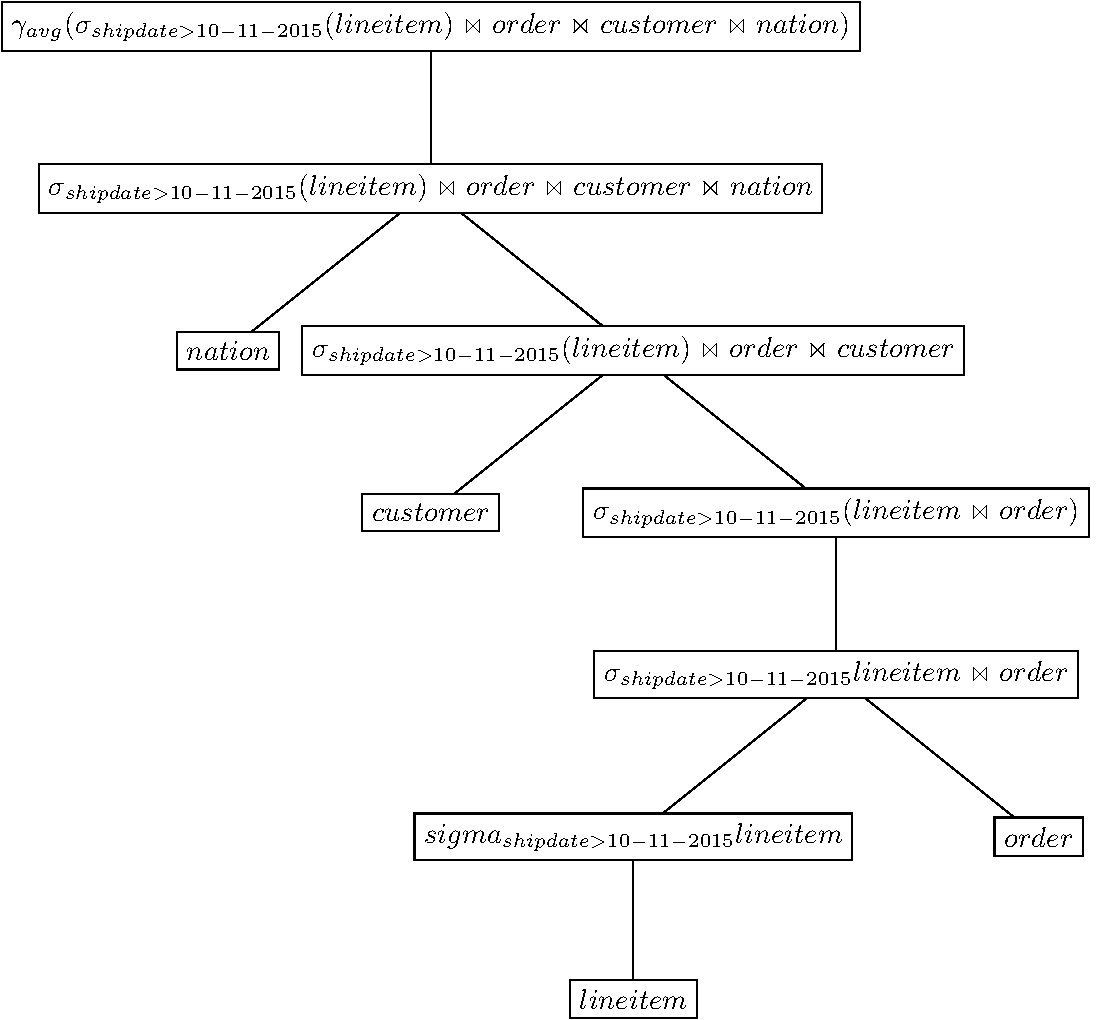
\includegraphics[width=.9\linewidth]{./imgs/optplan.pdf}
  \caption{\label{fig:optplan}A possible optimal plan for an isolated
    query.}
\end{figure}

However, for certain workloads, it might be beneficial to opt for
a plan that materializes the relation \(lineitem \Join order\) and the
relation \(customer \Join nation\) so they can be used to optimize
later queries. In that case, even if the most beneficial plan for the
isolated query is deemed to be the one shown in figure \ref{fig:optplan},
taking a holistic view of a workload during query planning making
heavy use of \(lineitem \Join order\) and \(customer \Join nation\) a
better choice would be what appears in figure \ref{fig:workplan}.

\begin{figure}[H]
  \centering
  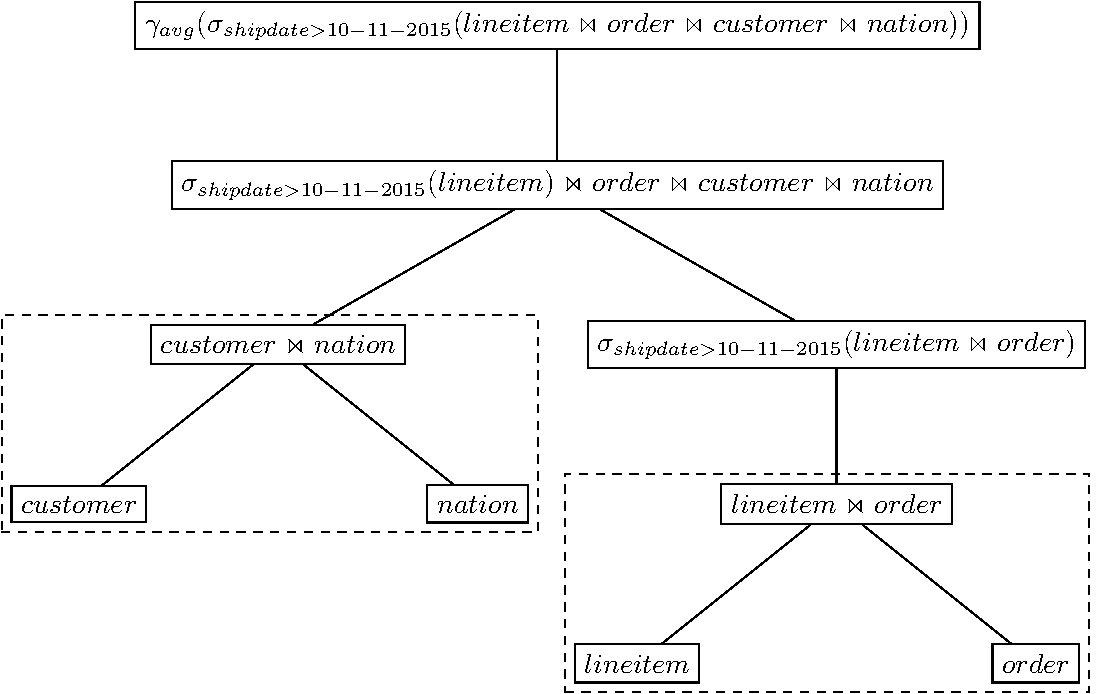
\includegraphics[width=.9\linewidth]{./imgs/workplan.pdf}
  \caption{\label{fig:workplan}A possible optimal plan for a sequence
    of queries that makes heavy use of \(lineitem \Join order\) and
    \(customer \Join nation\)}
\end{figure}

A simple but effective solution to addressing the problem of
integrating incremental query materialization and the optimization
processes, was presented in
\cite{perezHistoryawareQueryOptimization}. In their approach they
maintain a \emph{history pool} (a list of all the past queries) that is
used to decide the benefit of materializing a sub-expression, and a
\emph{view pool} that keeps track of the materialized tables at every
moment. Both these sets are taken into account during planning to
produce a plan that will likely minimize the amortized cost of the
workload. After the query is solved the sets are updated. A limitation
of such an approach is that when dealing with relations like
\(lineitem \Join order\) in budget restricted settings, materialized
view storage can quickly become a scarce resource.

There is an opportunity to reduce the effect of this problem by
exploiting another common workload attribute: certain tables are
frequently subsumed by the same intermediate result. In the case of
our example it may be the case that, within our hypothetical workload,
whenever the \(lineitem\) or the \(order\) tables are encountered in a
query, they can usually be subsumed by the \(lineitem \Join order\)
relation. In other words, when both \(lineitem \Join order\) and
\(lineitem\) (or \(order\)) are materialized it is preferable to only use
\(lineitem \Join order\) in the query plan. Since most of the data of
\(lineitem\) and \(order\) are also in \(lineitem \Join order\), it might
make sense, instead of maintaining the \(lineitem\) and \(order\) tables
separately, to keep \(lineitem \Join order\) and enough information to
reconstruct \(lineitem\) or \(order\) when needed.

We propose a solution to both those problems resembles the solution
provided in \cite{gouSupSearchEfficient2006} by Gou et.al. In their work
they embed aggregations \sql{group by x1, .., xk} into the
\(\subseteq\)-lattice that arises from the powerset \(P(\{x_1, ...,
x_k\})\). Thereby they encode the fact that \sql{group by A, B, C} is
subsumed, or can be computed by, either of \sql{group by A, B}, \sql{group by
  A, C} or \sql{group by B, C}. Once the lattice is constructed a variant of
the \(A^{\star}\) path finding is used algorithm to search for the
optimal aggregation plan. However \cite{gouSupSearchEfficient2006} on
the one hand makes no attempt to recycle tables, ie. garbage collect
tables, whose data can be found in other relations, and narrows it's
attention to aggregations.

From the aforementioned work we keep the basic notion of using a graph
to represent the subsumption of queries and to derive the benefit of
materializing a relation. We also use path finding techniques in that
graph to create plans. However we introduce a more complex and ad-hoc
hierarchy of relations to account for subsumptions the entire
relational algebra, rather than just aggregations that is very similar
to AND-OR dags as found in
\cite{mistryMaterializedViewSelection2001}. Thereby we express for
example the fact that \(\sigma_p(S)\) subsumes \(\sigma_{p \lor q}(S)\),
or that \(B \Join C\) subsumes \(A \Join B \Join C\). Furthermore the
relations we express in that graph are bidirectional. So rather than
only finding paths towards the goal and deleting relations when they
are no longer needed, we simultaneously plan for moving towards the
goal query and performing "backwards" operations for saving up
space. We clarify this with an example which demonstrates a slightly
simplified version of our system's functionality.

In figure \ref{fig:intro_selectexample} we provide representation of a subsumption
graph that our RDBMS might create after witnessing selections on
\(lineitem\). For brevity let \(p:=shipdate > 10-11-2015\),
\(q:=quantity < 24\) and \(r:=discount < .06\). The RDBMS has
encountered \(\sigma_{p}(lineitem)\), \(\sigma_{q}(lineitem)\) and
\(\sigma_{q} \sigma_{r} (lineitem)\).

\begin{figure}[H]
  \centering
  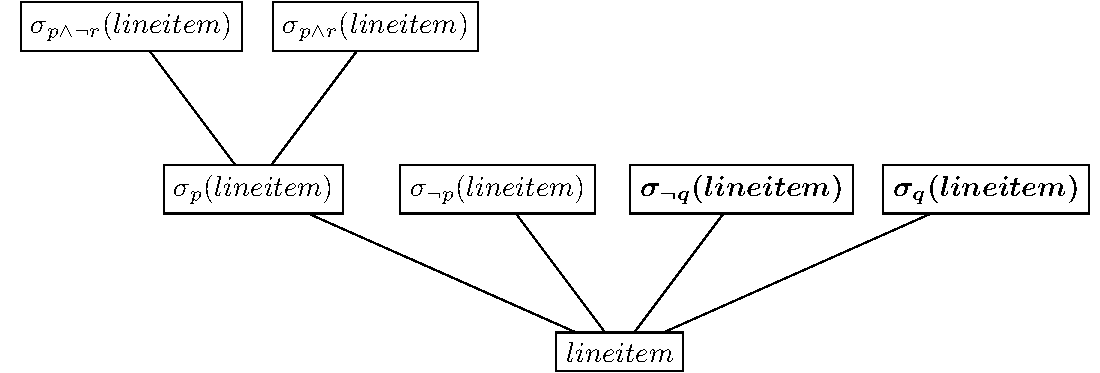
\includegraphics[width=.9\linewidth]{./imgs/intro_selectexample.pdf}
  \caption{\label{fig:intro_selectexample}Any relation can be selected
    in different ways forming a tree can be further split on top of
    that.}
\end{figure}

With \(\boldsymbol{bold}\) we mark the materialized relations. The query
that we are solving is \(\sigma_{quantity < 24} \sigma_{discount < .06}
(lineitem)\), which is denoted in the figure as \(\sigma_{q \land
  r}(lineitem)\). Our total size budget is 2.5.

Following the edges in the graph, to solve \(\sigma_{q \land
  r}(lineitem)\) we need \(\sigma_{q}(lineitem)\) and for that we need
\(lineitem\). So first the union:

\[
  \sigma_{\neg p}(lineitem) \cup \sigma_{p}(lineitem) \rightarrow lineitem
\]

Then we need \(\sigma_{q}(lineitem)\) but we are now using 2 units of
space and adding .6 more would exceed our space budget of
2.5. \(lineitem\) is the least beneficial of our materialized views
but it is required for our next step, ie. creating
\(\sigma_{q}(lineitem)\) . \(\sigma_{\neg p}(lineitem)\) is deleted
since it's derivable from \(lineitem\) and is least beneficial. Then
\(\sigma_{q}(lineitem)\) is created and now we are using 2.1 units of
space.

\[
  lineitem \rightarrow \sigma_{q}(lineitem)
\]

Finally we need to create the final relation \(\sigma_{q \land
  r}(lineitem)\) . However it's space requirement is .5 and we we would
be exceeding our budget. We can't delete \(lineitem\) even though it
is our least beneficial table because we would have no way of
recreating it.

Here we have two options. One is to delete \(\sigma_{\neg
  p}(lineitem)\), our most benefit al table. The other, which is the one
that the system should opt for, is to backtrack. When we created
\(\sigma_{q}(lineitem)\), instead we create both
\(\sigma_{q}(lineitem)\) and \(\sigma_{\neg q}(lineitem)\).

\[
  lineitem \rightarrow \{\sigma_{q}(lineitem), \sigma_{\neg q}(lineitem)\}
\]

Once both those tables are materialized we can safely delete
\(lineitem\). Now our space usage is 1.1 and we can safely

\[
  \sigma_{q}(lineitem) \rightarrow \sigma_{q \land r} (lineitem)
\]

Which is the requested query and, in summary, the final plan is:

\begin{align*}
  &\sigma_{\neg p}(lineitem) \cup \sigma_{p}(lineitem) \rightarrow lineitem \\
  &Delete[\sigma_{\neg p}(lineitem)] \\
  &lineitem \rightarrow \{\sigma_{q}(lineitem), \sigma_{\neg q}(lineitem)\} \\
  &Delete[lineitem] \\
  &\sigma_{q}(lineitem) \rightarrow \sigma_{q \land r} (lineitem)
\end{align*}

The key idea behind this work
is that a) by using reversible operations between relations and b) by
integrating the query planner and the materialized view recycling
mechanism, we get grater flexibility to adapt the data layout to the workload thereby
optimizing the use of our space budget.
